%%%%%%%%%%%%%%%%%%%%%%%%%%%%%%%%%%%%%%%%%
% Short Sectioned Assignment
% LaTeX Template
% Version 1.0 (5/5/12)
%
% This template has been downloaded from:
% http://www.LaTeXTemplates.com
%
% Original author:
% Frits Wenneker (http://www.howtotex.com)
%
% License:
% CC BY-NC-SA 3.0 (http://creativecommons.org/licenses/by-nc-sa/3.0/)
%
%%%%%%%%%%%%%%%%%%%%%%%%%%%%%%%%%%%%%%%%%

%----------------------------------------------------------------------------------------
%	PACKAGES AND OTHER DOCUMENT CONFIGURATIONS
%----------------------------------------------------------------------------------------

\documentclass[paper=a4, fontsize=11pt]{scrartcl} % A4 paper and 11pt font size

\usepackage[utf8]{inputenc}
\usepackage{fourier} % Use the Adobe Utopia font for the document - comment this line to return to the LaTeX default
\usepackage[portuguese]{babel} % English language/hyphenation
\usepackage{amsmath,amsfonts,amsthm} % Math packages
\usepackage{graphicx}

\usepackage{lipsum} % Used for inserting dummy 'Lorem ipsum' text into the template
\usepackage{url}
\usepackage[colorlinks=true]{hyperref}

\usepackage{sectsty} % Allows customizing section commands
\allsectionsfont{\centering \normalfont\scshape} % Make all sections centered, the default font and small caps

\usepackage{fancyhdr} % Custom headers and footers
\pagestyle{fancyplain} % Makes all pages in the document conform to the custom headers and footers
\fancyhead{} % No page header - if you want one, create it in the same way as the footers below
\fancyfoot[L]{} % Empty left footer
\fancyfoot[C]{} % Empty center footer
\fancyfoot[R]{\thepage} % Page numbering for right footer
\renewcommand{\headrulewidth}{0pt} % Remove header underlines
\renewcommand{\footrulewidth}{0pt} % Remove footer underlines
\setlength{\headheight}{13.6pt} % Customize the height of the header

\numberwithin{equation}{section} % Number equations within sections (i.e. 1.1, 1.2, 2.1, 2.2 instead of 1, 2, 3, 4)
\numberwithin{figure}{section} % Number figures within sections (i.e. 1.1, 1.2, 2.1, 2.2 instead of 1, 2, 3, 4)
\numberwithin{table}{section} % Number tables within sections (i.e. 1.1, 1.2, 2.1, 2.2 instead of 1, 2, 3, 4)

\setlength\parindent{0pt} % Removes all indentation from paragraphs - comment this line for an assignment with lots of text

%----------------------------------------------------------------------------------------
%	TITLE SECTION
%----------------------------------------------------------------------------------------

\newcommand{\horrule}[1]{\rule{\linewidth}{#1}} % Create horizontal rule command with 1 argument of height

\title{	
\normalfont \normalsize 
\textsc{InfoLab---Faculdade de Engenharia da Universidade do Porto} \\ [25pt] % Your university, school and/or department name(s)
\horrule{0.5pt} \\[0.4cm] % Thin top horizontal rule
\huge Descrição de dados no Dendro\\ usando Dublin Core e descritores específicos de domínios \\ % The assignment title
\horrule{2pt} \\[0.5cm] % Thick bottom horizontal rule
}

\author{João Rocha da Silva} % Your name

\date{\normalsize\today} % Today's date or a custom date

\begin{document}

\maketitle % Print the title

%----------------------------------------------------------------------------------------
%	Introduction
%----------------------------------------------------------------------------------------

\begin{center}
	Contact:\\\url{joaorosilva@gmail.com}
\end{center}

\section{A experiência de avaliação do Dendro}

O Dendro é uma plataforma para depósito e partilha de dados gerados em projetos de investigação. O seu objetivo é ajudar os investigadores no processo de preparar os seus dados para serem arquivados num repositório de dados e eventualmente partilhados com outros investigadores.

Nesta experiência cada participante  vai assumir o papel de um ``curador'', ou seja um especialista encarregado de preparar dados para depósito. São obrigações do curador:
\begin{itemize}
\item Criar pastas para organizar os dados;
\item Carregar ficheiros com dados (texto, imagens, folhas de cálculo) nas pastas;
\item Fazer a descrição dos dados em cada pasta.
\end{itemize}

Na experiência o curador vai receber várias \emph{tarefas}. Numa tarefa procede-se à preparação de um ou mais conjuntos de dados. O trabalho do curador nesta experiência é atribuir metadados. O modelo de metadados usado é o Dublin Core, uma norma internacional de descrição ( ISO 15836) usada em todo o tipo de recursos. Nesta experiência iremos também disponibilizar alguns conjuntos de descritores extra, especialmente concebidos para captar os detalhes específicos do domínio de investigação de cada conjunto de dados. Em suma:
\begin{itemize}
	\item Dublin Core $\rightarrow$ Metadados genéricos
	\item Outros descritores $\rightarrow$ Metadados específicos de cada domínio
\end{itemize}

Para a criação dos metadados cada curador vai fazer as pesquisas necessárias sobre os dados que estiver a tratar para definir os metadados apropriados. 

Como o Dendro é um sistema em desenvolvimento, podem ocorrer erros. Perante uma situação em que o sistema não se comporte conforme esperado, o participante deve enviar uma mensagem ao contacto técnico. Esta mensagem deve explicar asituação em que ocorreu o problema, referir as mensagens de erro se for o caso e se possível incluir instruções sobre como repetir o erro.

O trabalho é realizado em grupos de 3 participantes; cada grupo comporta-se numa tarefa como um grupo de investigação na área escolhida para a tarefa. 

\begin{center}
	\textbf{Cada participante vai manter um diário das suas sessões com o sistema, para apresentar como anexo do relatório do trabalho prático.}
\end{center}

%------------------------------------------------

%----------------------------------------------------------------------------------------
%	Registration and creating a new project
%----------------------------------------------------------------------------------------

%\clearpage
\section{Registo e criação de um projeto}

O Dendro a usar nas tarefas é um dos seguintes:

\begin{center}
	\url{http://abd-mci.fe.up.pt:3007}. 
	
\end{center}
	
Aceda ao Dendro onde irá realizar o seu trabalho através do seu navegador Web (recomenda-se o Google Chrome em Windows ou o Safari no Mac OS X). 

\subsection{Não consigo aceder!} % (fold)
\label{sub:nao_consigo_aceder}

Se não conseguir aceder, verifique os seguintes pontos:

\begin{itemize}
	\item Está dentro da rede da FEUP? (eduroam)
	\item Se estiver em casa: Ligou a VPN da FEUP?
	\item Tem os servidores DNS em branco nas configurações IPV4 da sua ligação à rede, ou seja, não está a usar os servidores DNS da Google (8.8.8.8 / 8.8.4.4)?
\end{itemize}


% subsection nao_consigo_aceder (end)

\subsection{Registo / Autenticação no sistema}

\begin{figure}[h!t!]
	\centering
	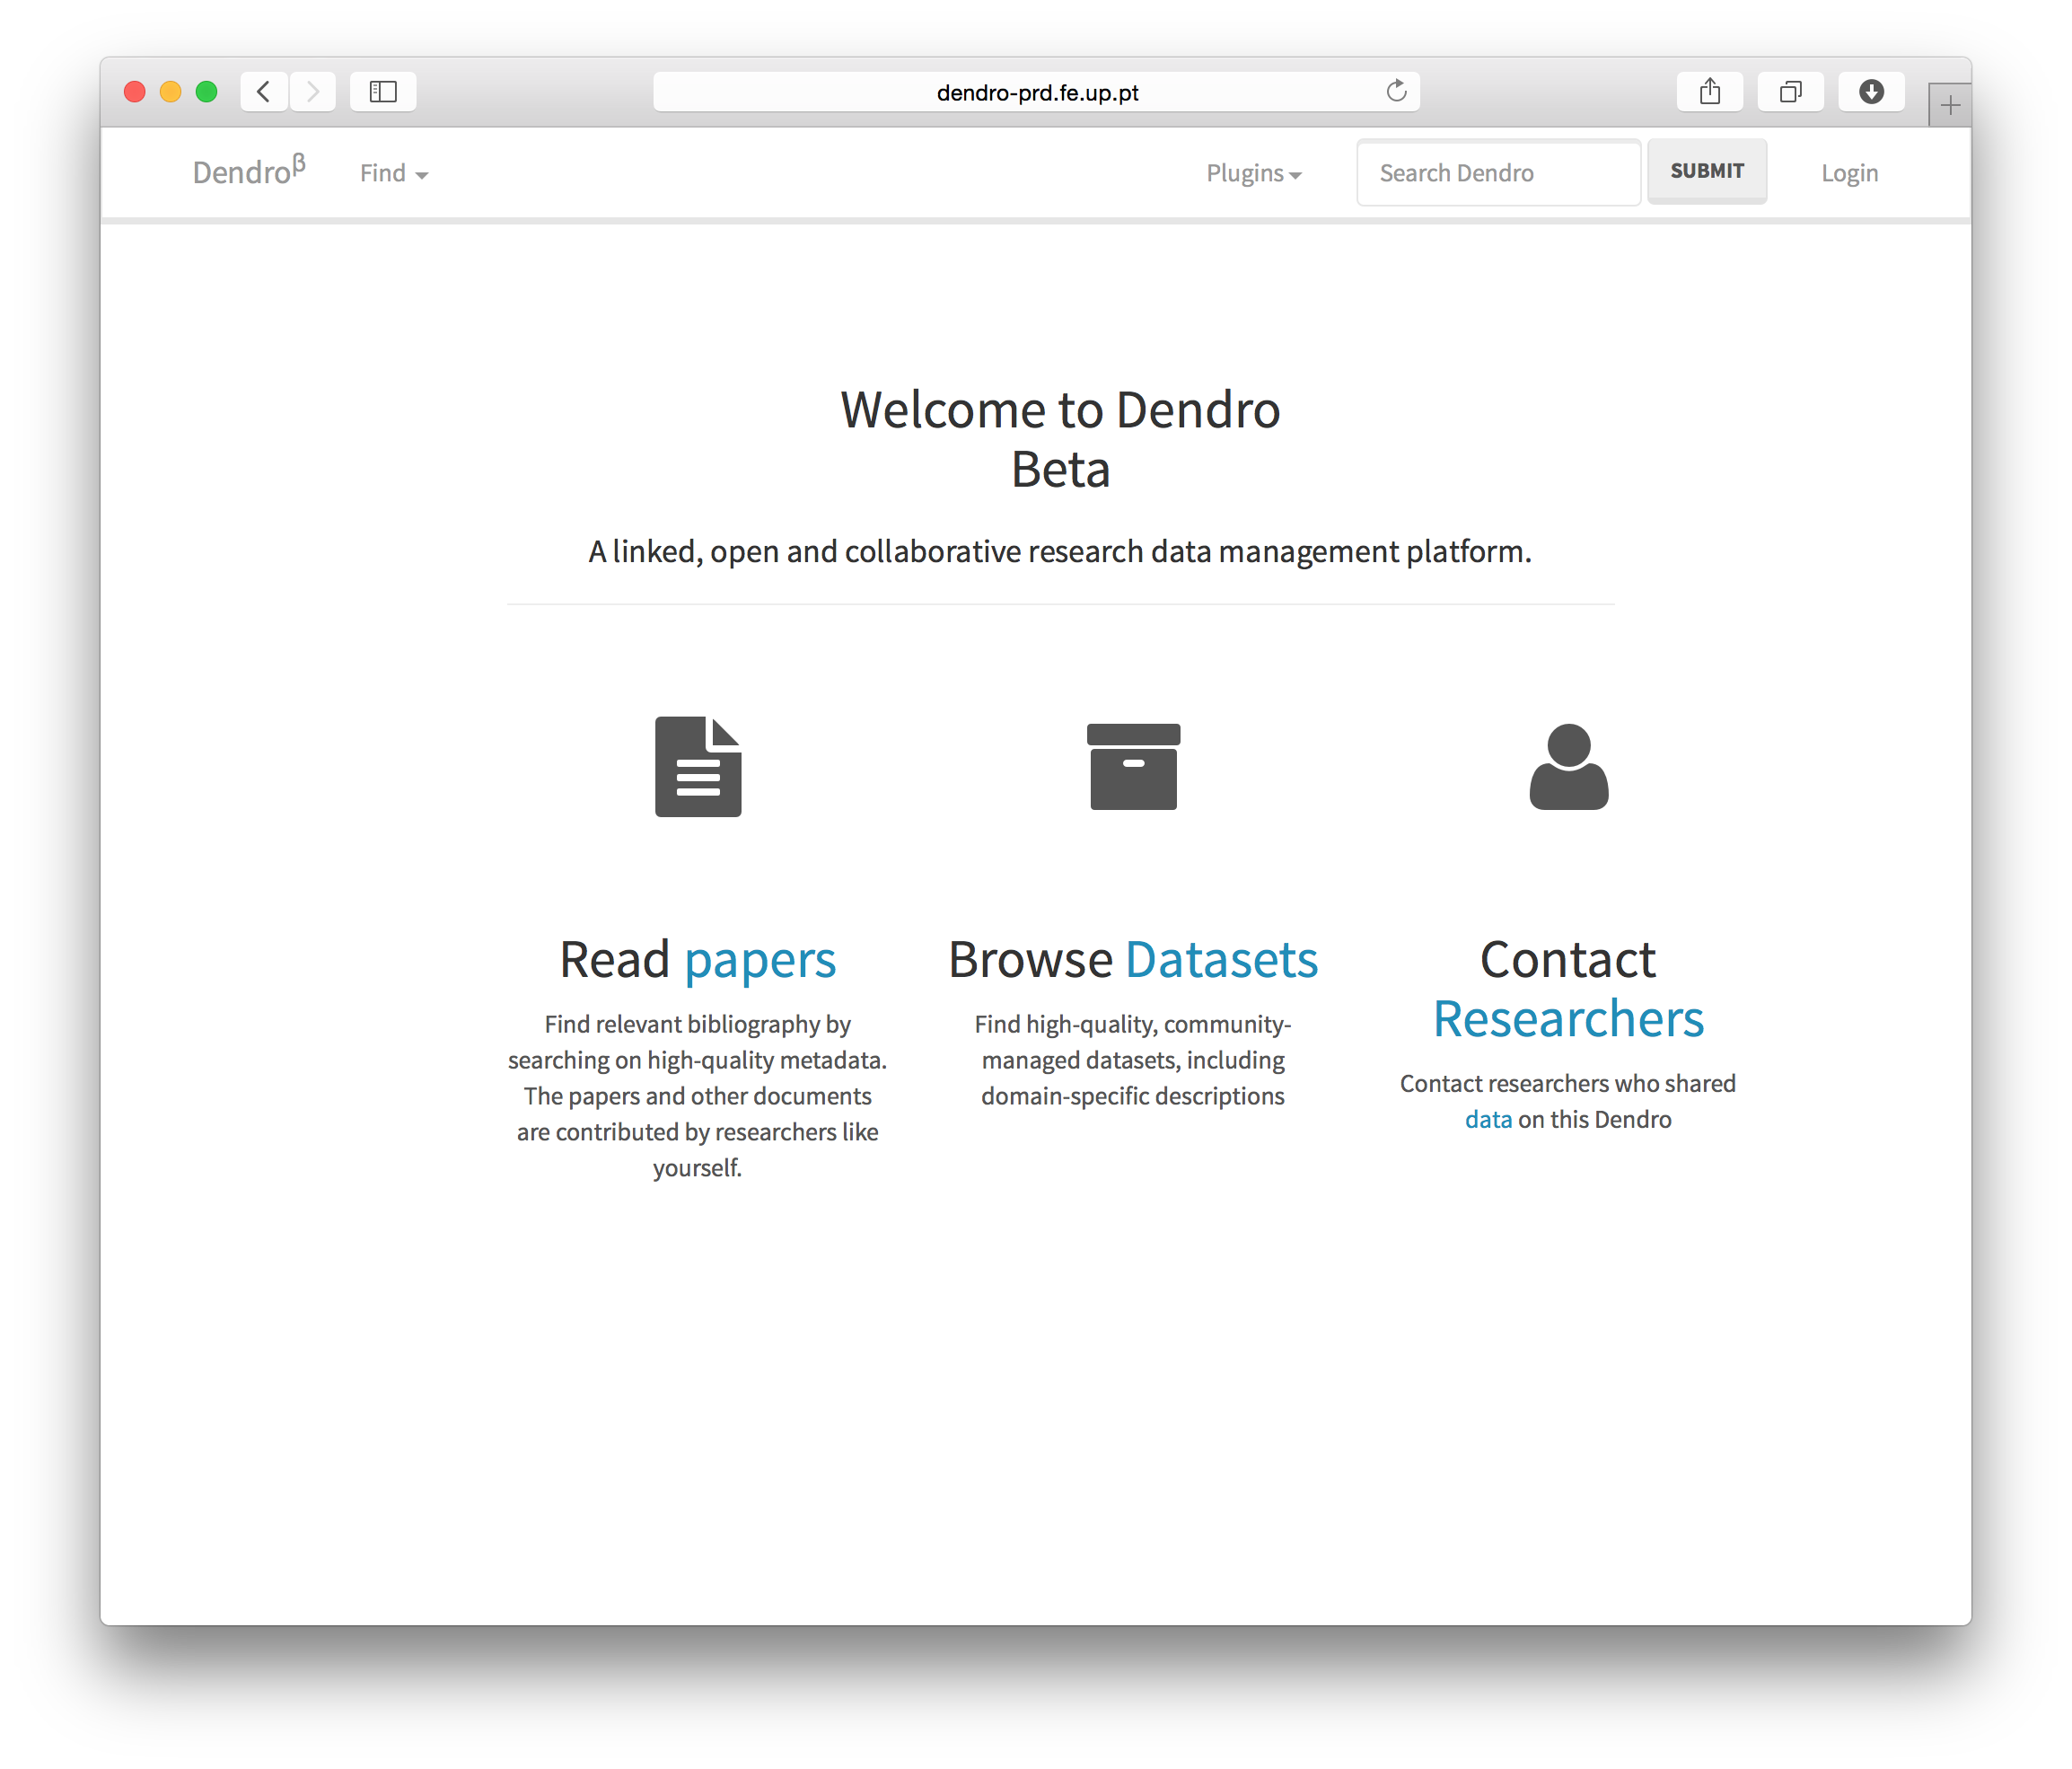
\includegraphics[width=\textwidth]{Images/homepage}
	\caption{A página inicial da plataforma Dendro}
	\label{fig:homepage}
\end{figure}

A página inicial da plataforma Dendro será semelhante à apresentada na Figura \ref{fig:homepage}\footnote{Os administradores da plataforma podem aplicar temas diferentes à plataforma, pelo que as cores e tipos de letra podem variar. No entanto, elementos de interface com o utilizador como botões e caixas de texto estarão sempre nos mesmos locais.}. Na barra do topo estão algumas funcionalidades importantes, que são aqui descritas brevemente (ordem da esquerda para a direita).

O título (nome da plataforma neste caso) permite voltar com 1 clique à página inicial do Dendro. Na lista de opções ``Find'' existem 3 opções: ``People'', que possibilita ao utilizador encontrar outros utilizadores já registados no sistema; ``Projects'', que permite aos utilizadores registados e autenticados no sistema encontrar projectos Dendro.

\begin{figure}[h!t!]
	\centering
	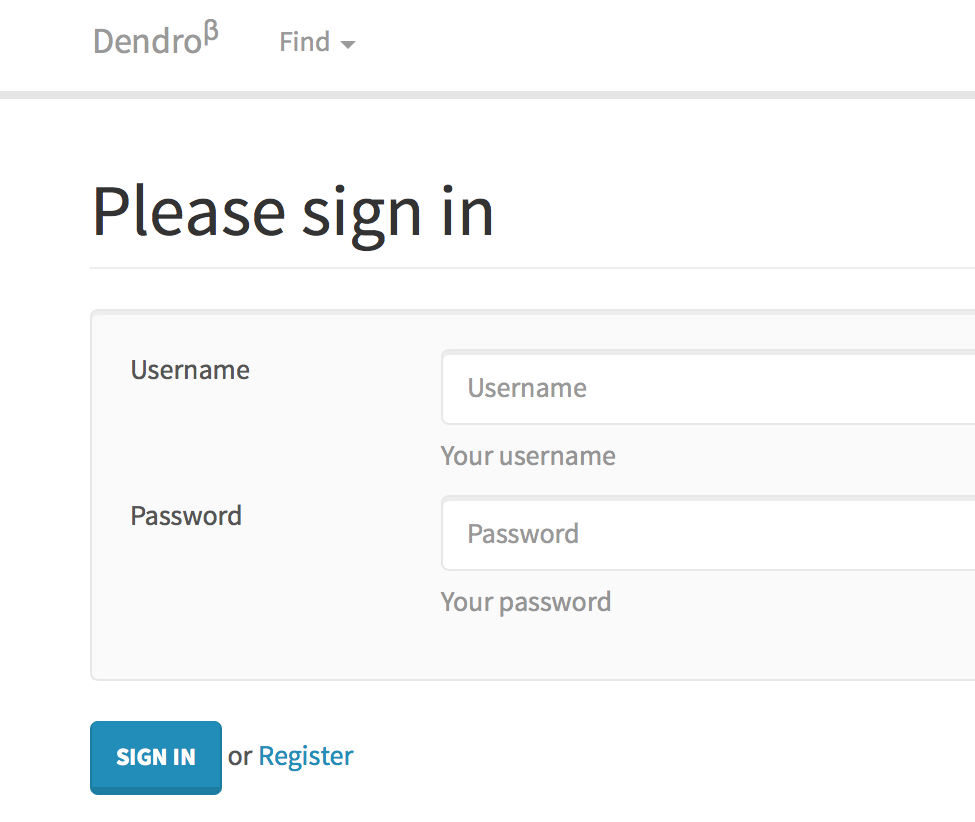
\includegraphics[width=0.4\textwidth]{Images/login}	
	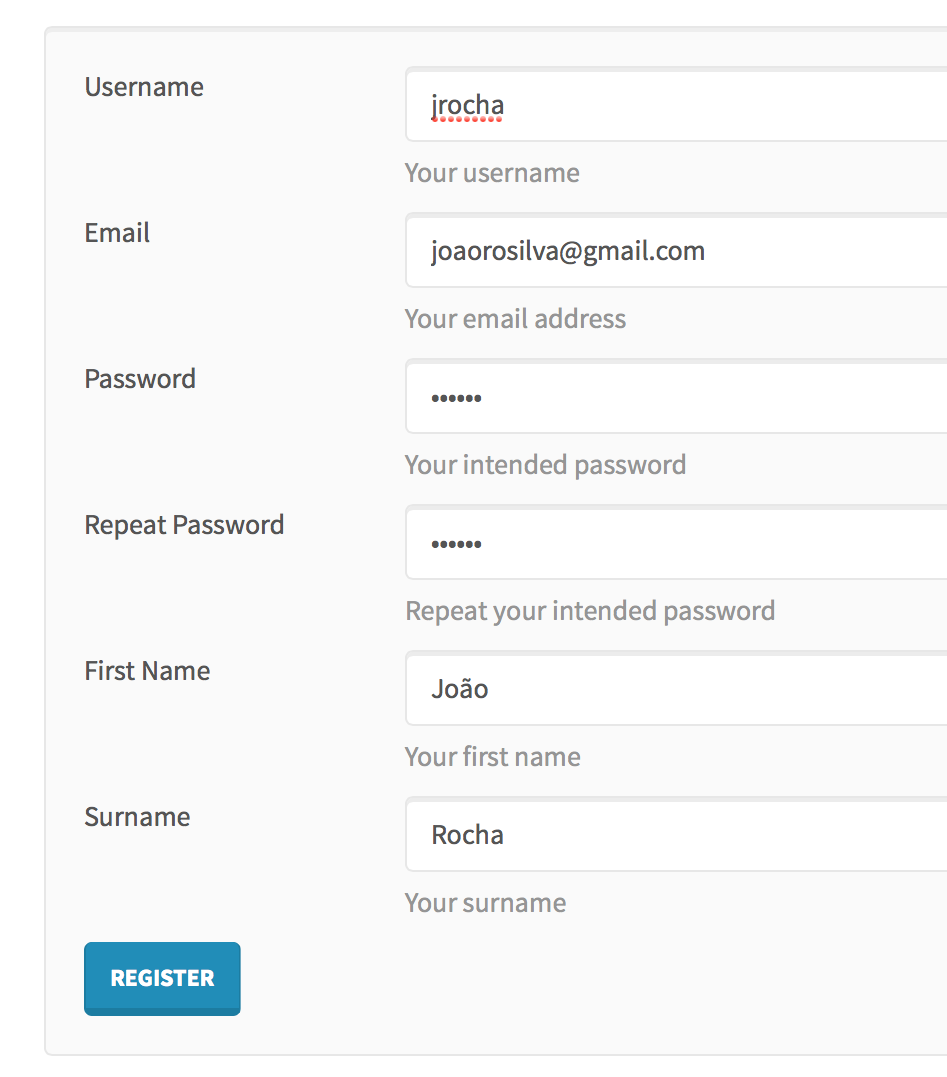
\includegraphics[width=0.4\textwidth]{Images/register}
	\caption{As páginas de autenticação e de registo na plataforma}
	\label{fig:login_and_register_pages}
\end{figure}

A opção mais à direita, ``Login'', permite aos utilizadores autenticarem-se no sistema. Seleccione essa opção; irá ver um ecrã que lhe pede para inserir o seu nome e senha (Figura\ref{fig:login_and_register_pages}). Insira as credenciais que lhe irão ser dadas para aceder ao sistema. A opção de registo de novos utilizadores (``Register'') deve ser usada para se registar, e deverá usar o seu login (por exemplo: up123456789), para facilitar a avaliação do trabalho.

Após a autenticação fica disponível a lista de projectos. É provável que, da primeira vez que se autentique, a lista esteja vazia, tal como mostra a figura~\ref{fig:empty_list_of_projects}. 

\begin{figure}[h!t!]
	\centering
	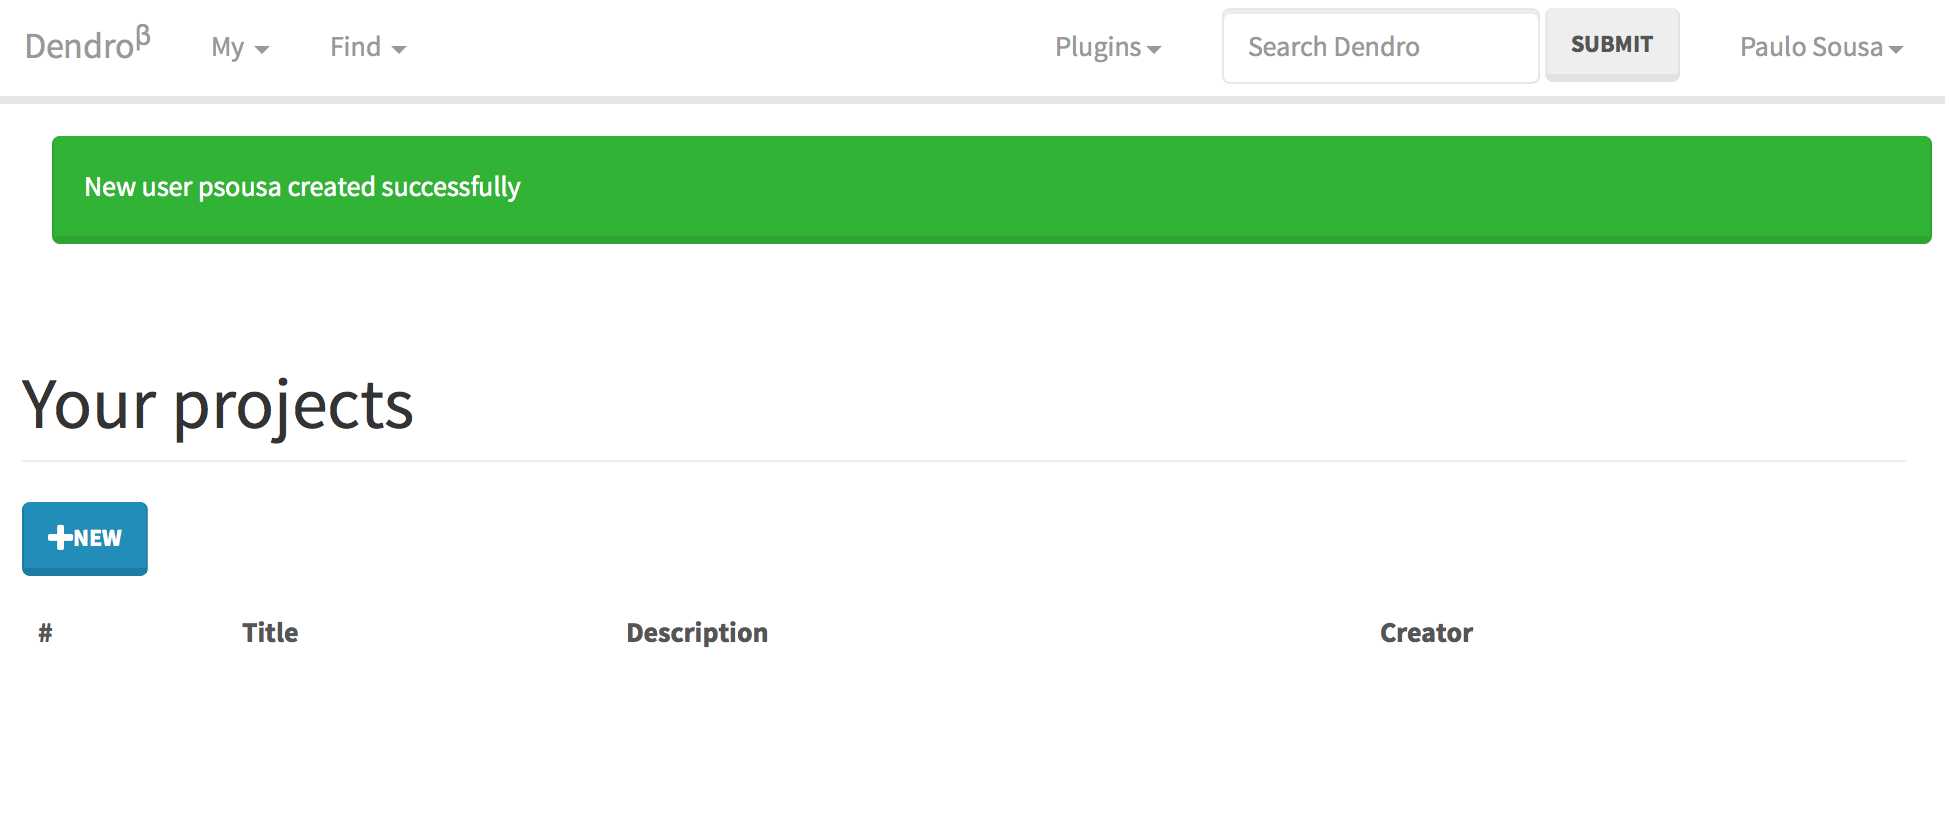
\includegraphics[width=0.8\textwidth]{Images/empty_list_of_projects}	
	\caption{Uma lista de projectos vazia}
	\label{fig:empty_list_of_projects}
\end{figure}

Crie um novo projecto seleccionando a opção ``New''. O sistema pedir-lhe-á alguma informação sobre o projecto. Tenha atenção à especificação do \emph{handle} do projecto. Este valor é usado internamente pelo Dendro para identificar unicamente o seu projecto no sistema, pelo que não poderá alterá-lo após ter criado o projecto. Os caracteres aceites num \emph{handle} são apenas alfanuméricos (palavras compostas por letras minúsculas ou números, sem caracteres especiais ou espaços). Preencha a restante informação e pressione o botão ``Create''. Após a criação do projecto, este será apresentado na sua lista de projectos (veja a Figura~\ref{fig:creating_a_project}).

\begin{figure}[h!t!]
	\centering
	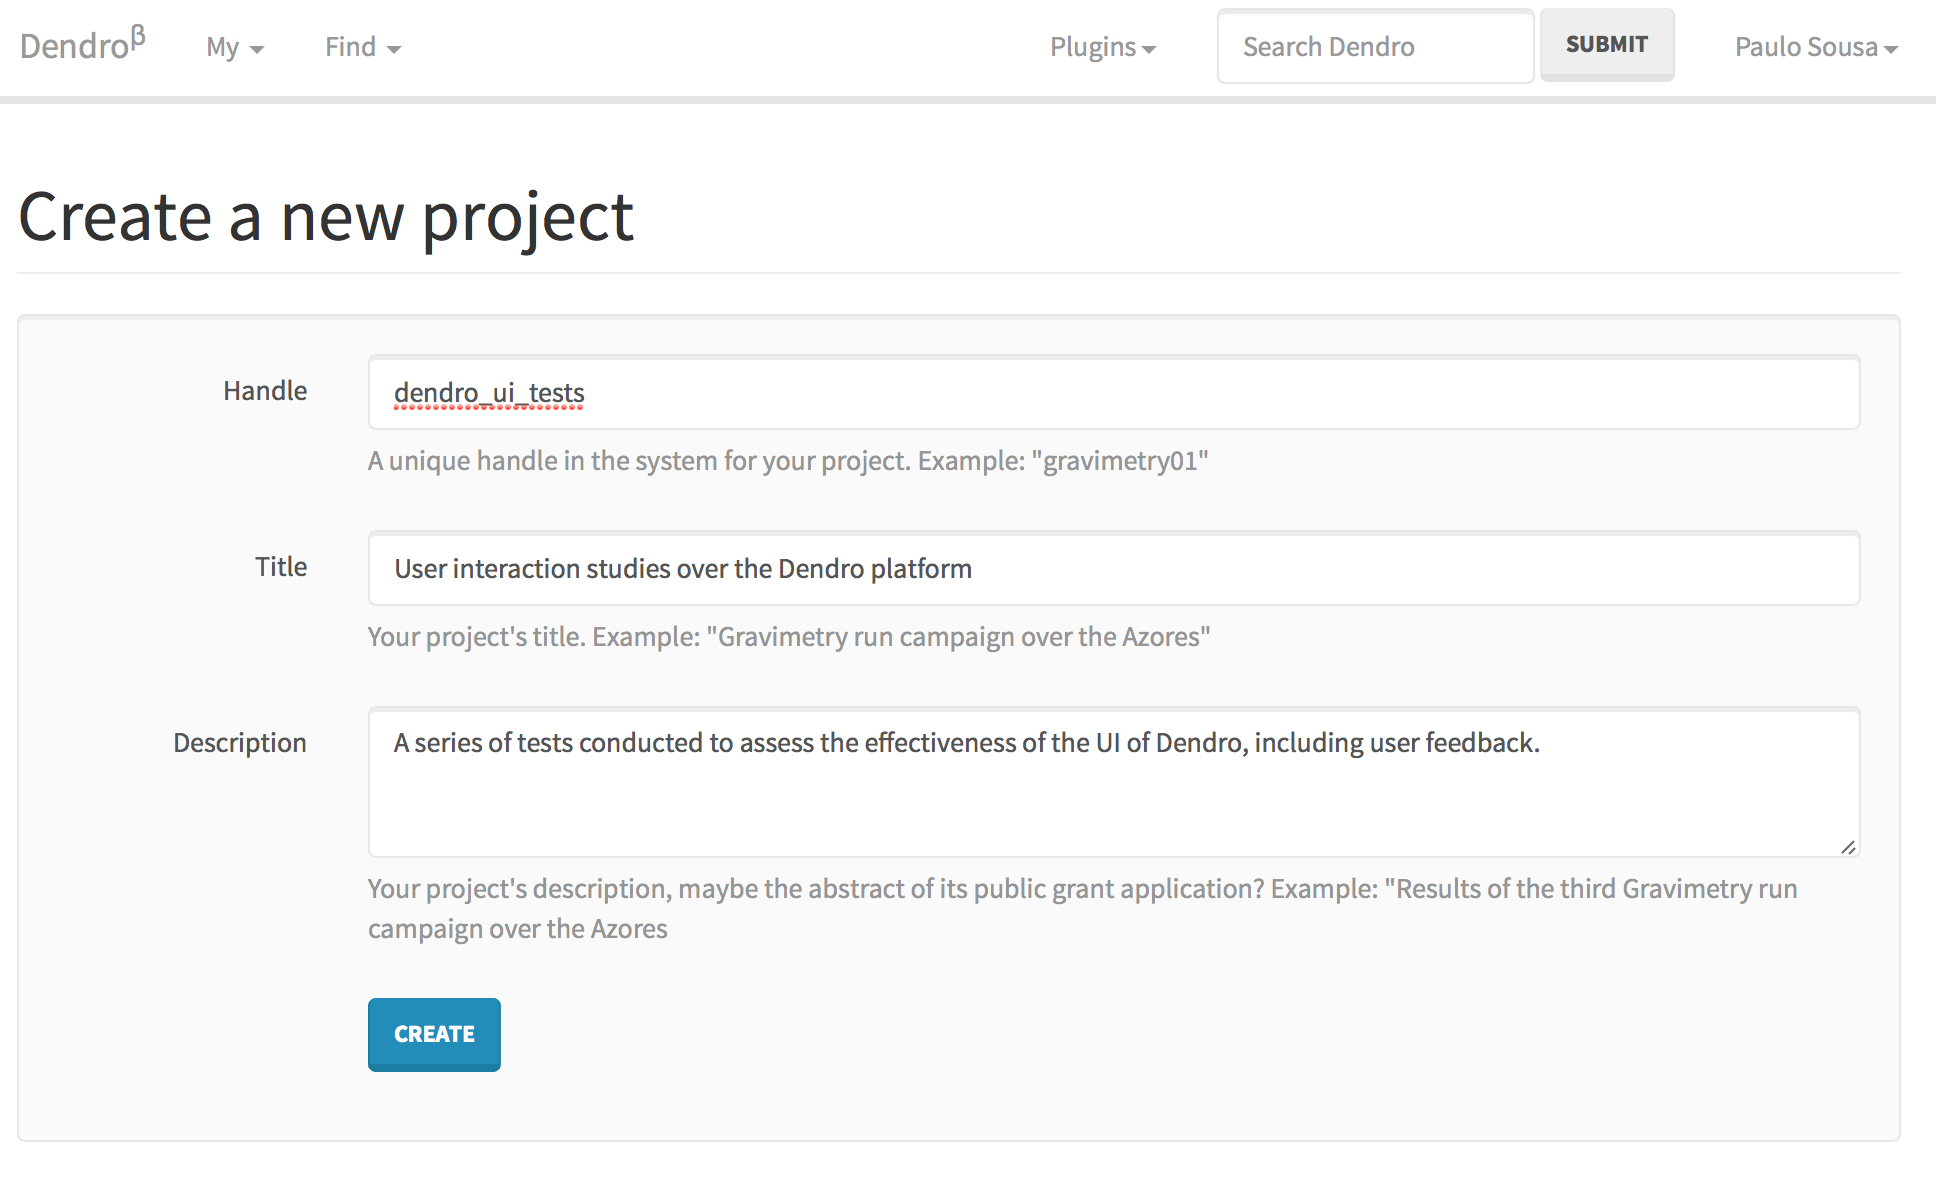
\includegraphics[width=0.8\textwidth]{Images/creating_a_project}	
	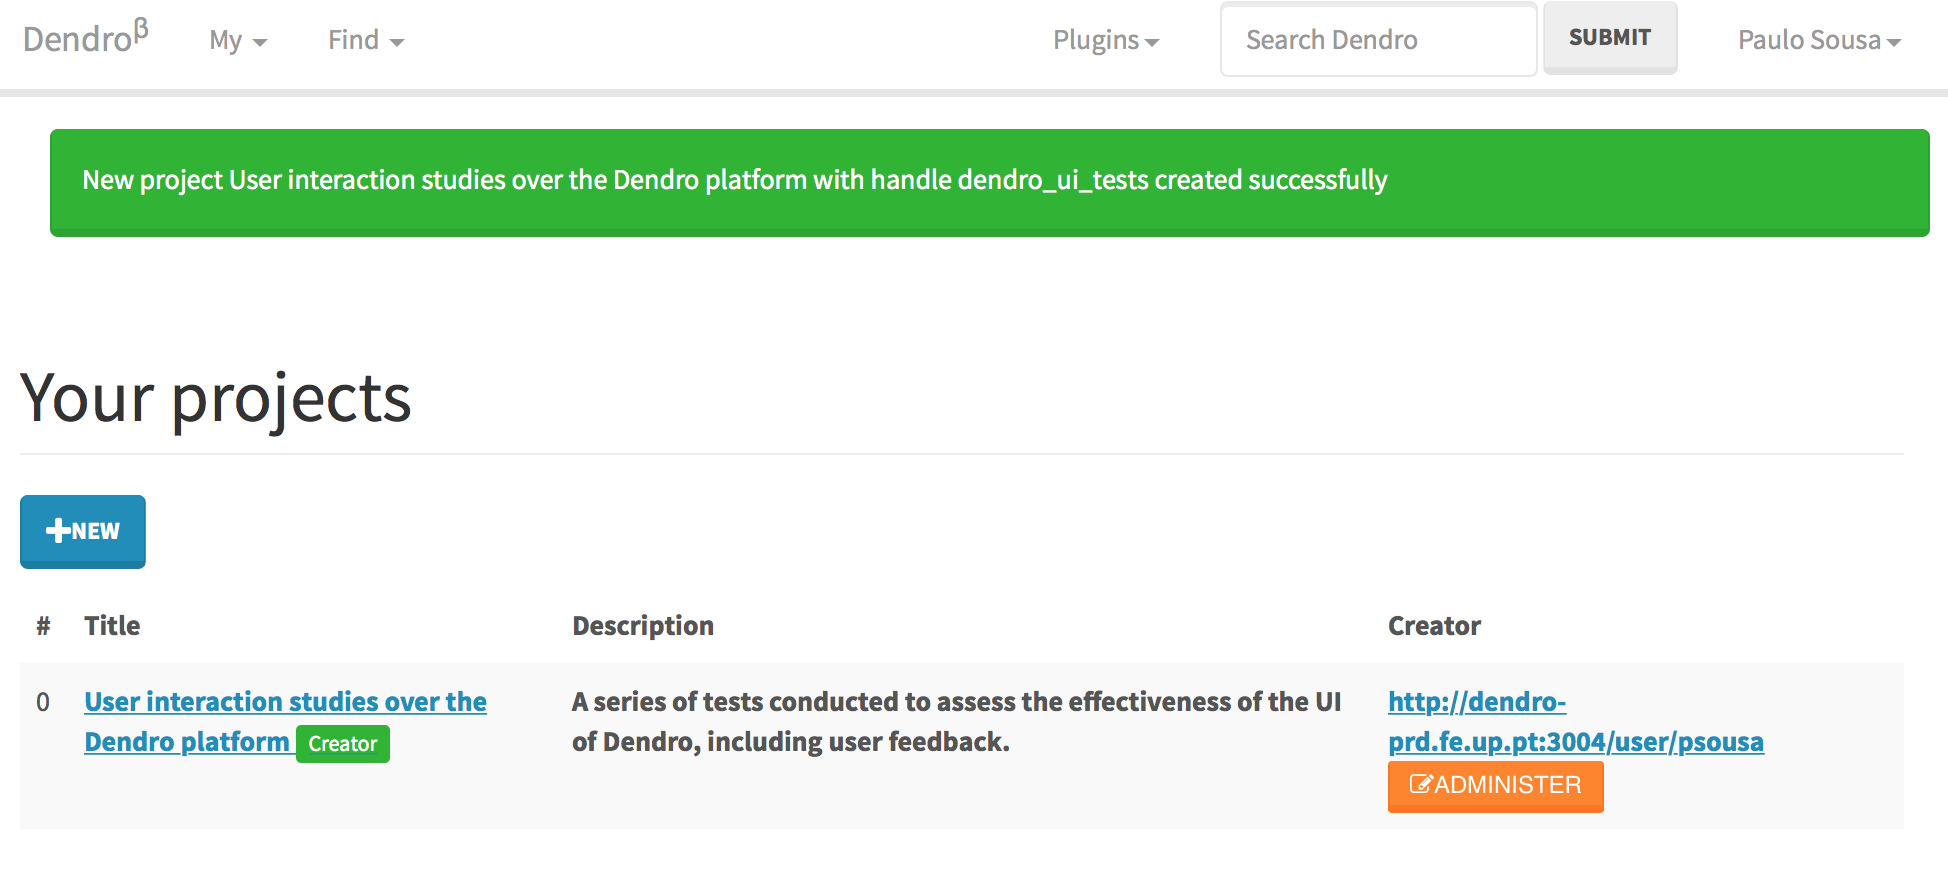
\includegraphics[width=0.8\textwidth]{Images/project_created}	
	\caption{Criação de um novo projecto}
	\label{fig:creating_a_project}
\end{figure}

\subsection{Administração de projecto---como adicionar colaboradores} % (fold)
\label{sub:project_administration}

Os criadores de um projecto verão um ícone com a palavra``Creator'' ao lado do título do mesmo. Para cada projecto que tenham criado também verão um botão ``Administer'' do lado direito. Os utilizadores que não tenham criado um projecto podem ser adicionados como colaboradores a um projecto já existente. Os colaboradores podem ver, na sua lista de projectos, os projectos nos quais colaboram. Também podem efectuar todas as operações descritas neste guia sobre o projecto, com a excepção de apagar o projecto e de o administrar (adicionar colaboradores, por exemplo). No caso do projecto que acabou de criar, o administrador será o próprio utilizador, portanto terá acesso ao botão ``Administer'' (Figura \ref{fig:administer_a_project}). Seleccione esta opção.

\begin{figure}[h!t!]
	\centering
	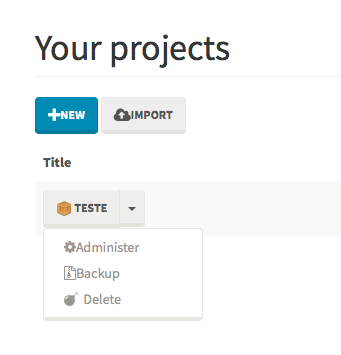
\includegraphics[width=0.3\textwidth]{Images/administer_project}	
	\caption{Administrar um projeto}
	\label{fig:administer_a_project}
\end{figure}

Esta área permite-lhe editar informação do projecto como o seu \emph{título} e a sua \emph{descrição}. Permite-lhe também \emph{adicionar colaboradores} ao projecto. Para adicionar um colaborador, seleccione o separador ``People'' e adicione o utilizador pretendido. Para encontrar o utilizador, escreva parte do seu nome, e o sistema deverá apresentar uma lista com sugestões (Figura \ref{fig:add_collaborators_to_a_project}). Depois de escolher o colaborador que pretende acrescentar, pressione Enter.

\begin{figure}[h!t!]
	\centering	
	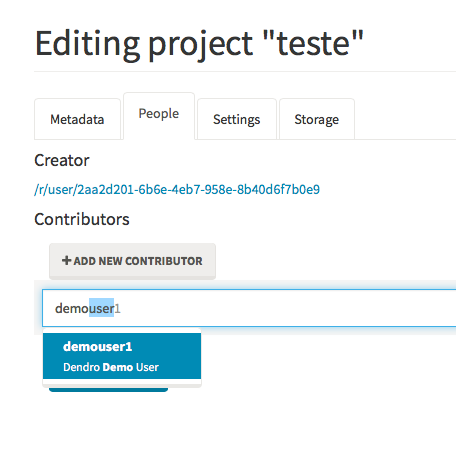
\includegraphics[width=0.3\textwidth]{Images/add_collaborators}	
	\caption{Adicionar colaboradores a um projeto}
	\label{fig:add_collaborators_to_a_project}
\end{figure}


%----------------------------------------------------------------------------------------
%	File management and metadata creation
%----------------------------------------------------------------------------------------

\section{Gestão de ficheiros e criação de metadados} % (fold)
\label{sec:managing_files_and_creating_metadata_records}

As interfaces principais da plataforma Dendro podem ser usadas para gerir ficheiros e pastas, assim como para produzir registos de metadados.

\subsection{Página do projeto} % (fold)
\label{sub:project_home_screen}

A Figura~\ref{fig:main_screen} mostra a interface principal do Dendro. Cada número na lista seguinte refere-se a uma área identificada nessa figura.

\begin{enumerate}
	\item \textbf{Operações sobre ficheiros}---Estes botões permitem aos utilizadores criar pastas, fazer o \emph{upload} e o \emph{download} de ficheiros, bem como outras opções para cópias de segurança.
	
	\item \textbf{Explorador de ficheiros}---Este explorador permite ao utilizador ver o conteúdo da pasta onde se encontra e navegar na hierarquia de pastas do projecto. Um clique sobre um item faz a seleção. Ao seleccionar um item, o utilizador pode ver os metadados  associados ao item; algumas operações adicionais ficam então disponíveis. Um duplo clique navega para a pasta escolhida. Para aceder à pasta imediatamente acima na hierarquia, o utilizador  selecciona o item no topo do explorador.
	
	\item \textbf{Estatísticas do projecto}---O painel de estatísticas mostra diversa informação relativas a projecto, tal como: o número de pessoas envolvidas, o número de pastas e ficheiros, o número de \emph{revisões}, ou seja versões dos registos de metadados que foram criados durante a vida do projecto. 
		
	\item \textbf{Menus de ``modo de edição'', partilha e exportação}---O botão Modo de Edição (``Edit Mode'') permite alternar entre uma interface adequada para a leitura e a consulta dos ficheiros depositados---com pré-visualização de alguns tipos de ficheiros como documentos, imagens ou áudio---e o modo de edição dos metadados para o recurso seleccionado no explorador de ficheiros. Os botões de partilha (``Share'') e de exportação dão acesso a algumas funções avançadas.
\end{enumerate}

\begin{figure}[h!t!]
	\centering
	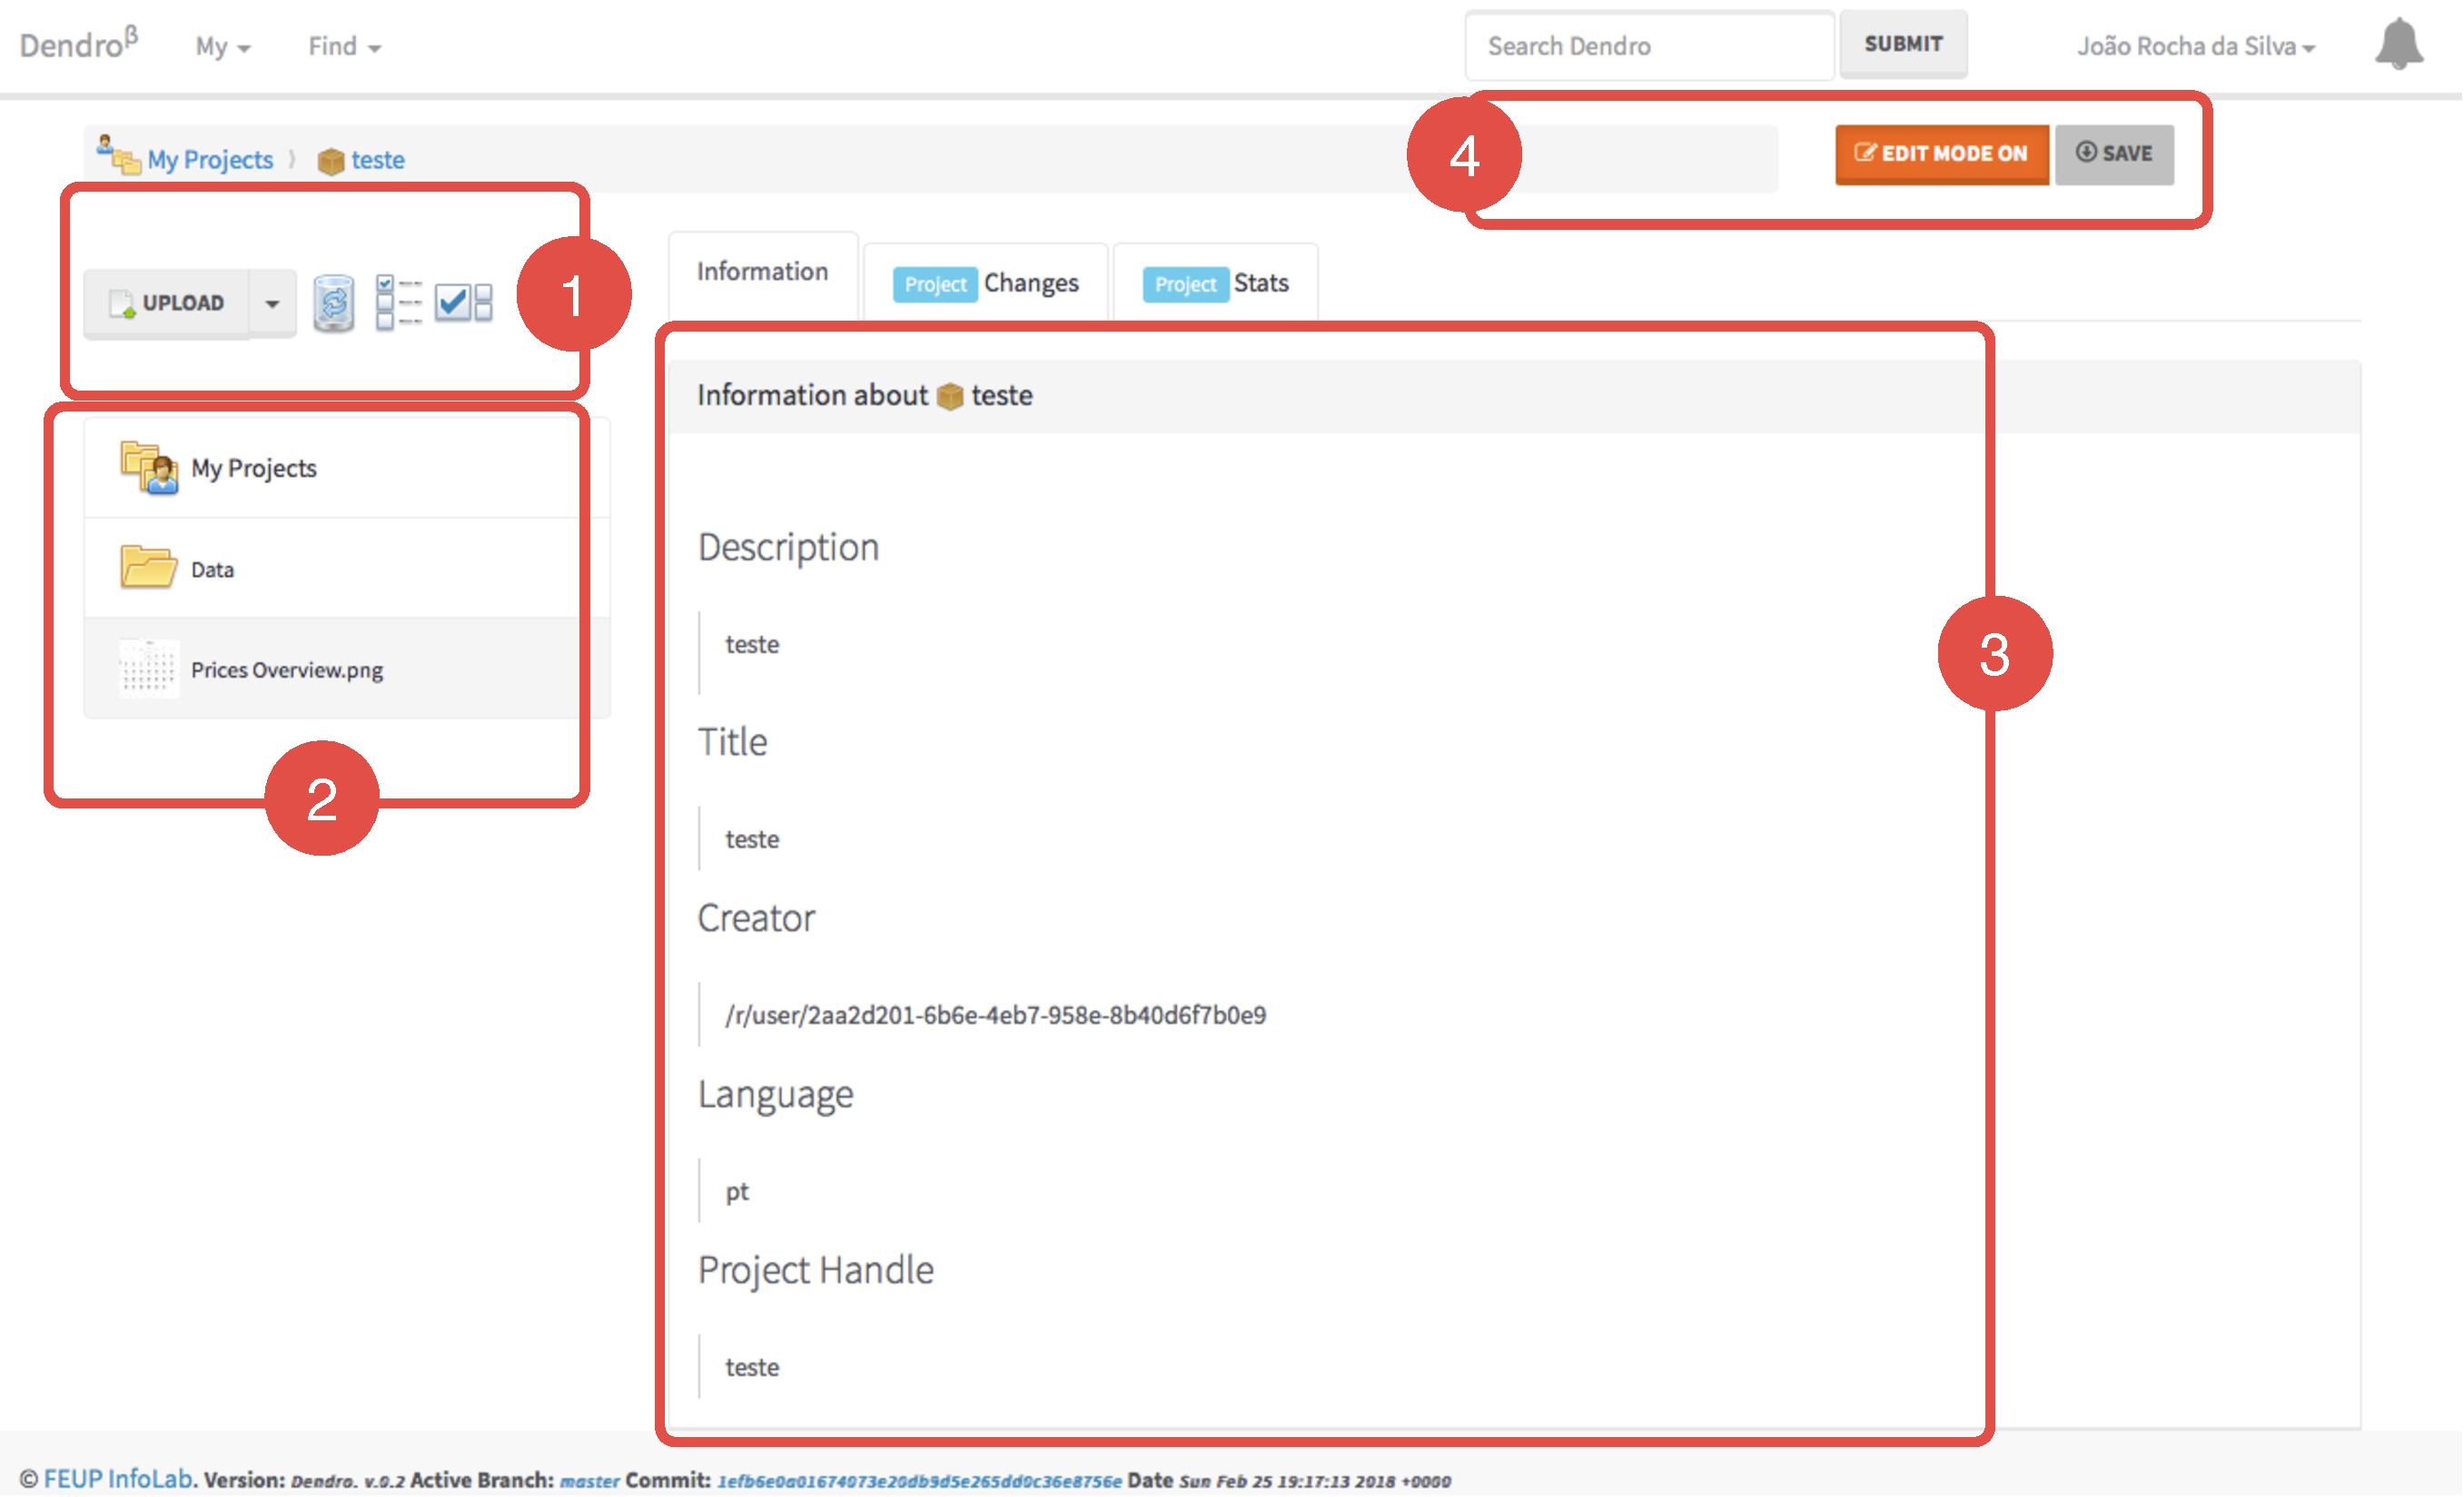
\includegraphics[width=\textwidth]{Images/main_screen}	
	\caption{Ecrã principal de gestão de dados da plataforma Dendro}
	\label{fig:main_screen}
\end{figure}

% subsection project_home_screen (end)

\subsection{Operações sobre ficheiros e pastas} % (fold)
\label{sub:basic_file_and_folder_operations}

Comece por adicionar uma pasta para os ficheiros que vai trazer para o Dendro. Pressione a seta à direita do botão ``Upload'' e seleccione ``Add folder'' e insira o nome para a nova pasta. Esta será criada e adicionada ao explorador de ficheiros à esquerda (\textbf{2}). Pode criar pastas adicionais se assim o entender.

Quando tiver acabado, faça um único clique sobre uma das pastas que criou, e depois faça clique direito sobre a pasta seleccionada. Deverão aparecer uma série de opções, incluindo apagar o item seleccionado. Se apagar o recurso, ele apenas fica escondido da primeira vez que o faz. O botão ``Show/Hide deleted items'' à direita do botão ``Upload''  permite esconder ou mostrar os items marcados como apagados. Ao escolher a opção ``Undelete'' do menu que aparece quando clica com o botão direito, poderá marcar o ficheiro como não apagado. Para apagar definitivamente, seleccione ``Really delete'' no menu que aparece ao clicar com o botão direito. 

Faça agora duplo clique sobre uma das pastas recém-criadas para navegar para dentro da mesma. A interface ao centro irá mudar para um ecrã que contém agora apenas 2 separadores: ``Information'' e ``Change Log'', sendo escondido o separador ``Stats''. Quando o separador ``Information'' está seleccionado,vemos uma lista dos valores dos metadados para o recurso selecionado no explorador à esquerda; selecionando o separador ``Change Log'' vemos o histórico de edições da ficha de metadados associada ao recurso. Caso não esteja selecionado um recurso, a informação apresentada é relativa à pasta actualmente aberta no explorador.

% subsection basic_file_and_folder_operations (end)

\subsection{Edição de metadados} % (fold)
\label{sub:editing_metadata}

Dado que as pastas que acabou de criar não possuem quaisquer metadados associados, irá ver uma mensagem que diz: \emph{This resource does not have any metadata yet. Add new descriptors in edit mode}. Para activar o modo de edição de metadados, faça clique sobre o botão ``Edit mode OFF'' no topo direito. A interface  muda para uma mais complexa, com as duas secções que vemos na Figura~\ref{fig:dendro_in_edit_mode}.

A área (\textbf{1}) mostra uma medida do preenchimento dos metadados associados à pasta. Dado que muitos investigadores produzem ficheiros de natureza similar, o botão (\textbf{2}) permite copiar os metadados da pasta imediatamente acima para o registo que estamos a tratar. Esta cópia permite associar os metadados comuns a todos os recursos dentro de uma pasta de forma  rápida: adicionam-se os metadados comuns ao nível da pasta e depois, para cada uma das pastas ou ficheiros abaixo, recorre-se a este botão para os copiar, mudando só o necessário para cada um dos recursos dentro da pasta.

\begin{figure}[h!t!]
	\centering
	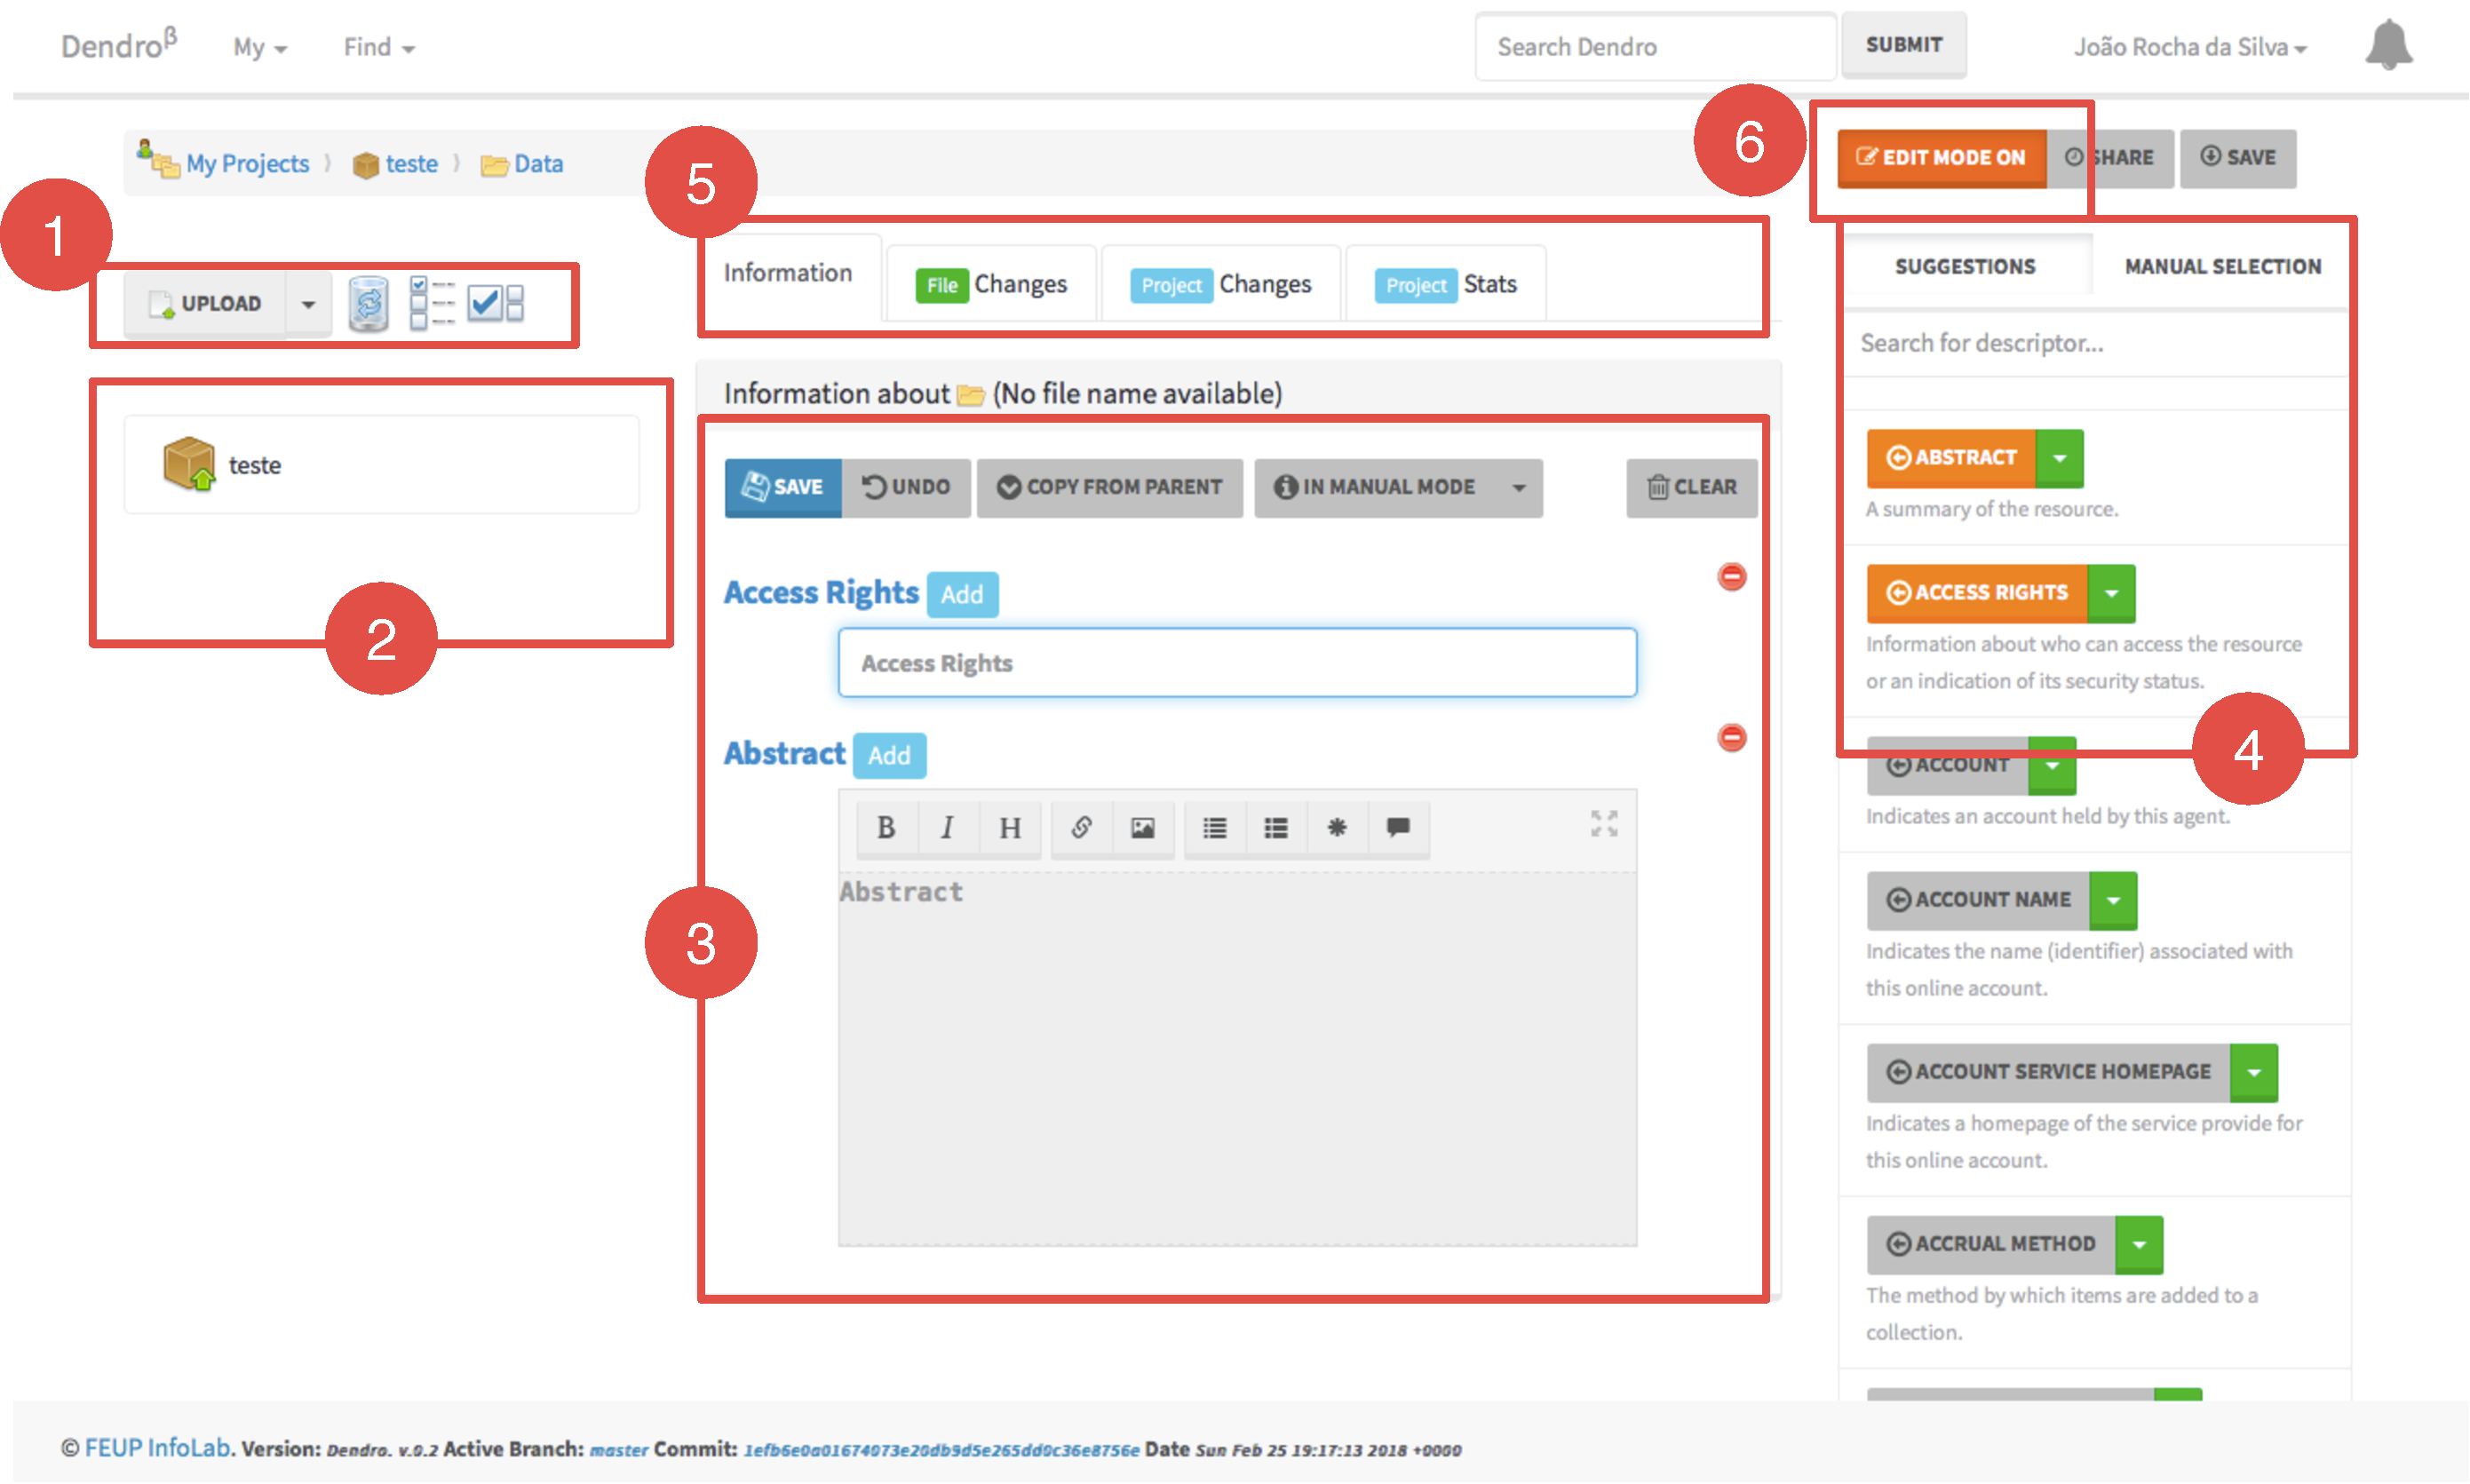
\includegraphics[width=\textwidth]{Images/in_edit_mode}	
	\caption{A página de edição de metadados (modo de edição activo)}
	\label{fig:dendro_in_edit_mode}
\end{figure}


%----------------------------------------------------------------------------------------
%	Task
%----------------------------------------------------------------------------------------

\section{Tarefas} % (fold)
\label{sec:tasks}

Na primeira semana do trabalho de avaliação vamos usar o Dendro, testar as funções descritas neste guião e fazer as primeiras descrições de dados de acordo com as tarefas especificadas.

As tarefas são organizadas por semanas e por grupos. Em cada semana, um grupo procura as suas tarefas na lista de tarefas (ver página das tarefas).



% FORA
%\subsubsection{Adding descriptors manually} % (fold)
%\label{ssub:adding_descriptors_manually}
%
%Using the right side menu (in area \textbf{4}) called ``Descriptor Selection'', you can search for metadata schemas from which to draw additional descriptors to complement your metadata sheets. Simply place your cursor on the text box and start typing. You will be able fo find descriptor sets based on their textual description and purpose, as well as their unique identifier. For example, typing ` ` ``dcterms'' and selecting the result from the auto-complete list, or typing a human-readable search phrase, such as ``generic'', will also yield the general-purpose \emph{Dublin Core Terms} metadata schema. Some schemas and their respective domains are shown in Table \ref{tab:schemas_overview}.
%
%\begin{table}[h!]
%  \begin{center}
%    \leavevmode
%	\begin{tabular}{|p{0.1\textwidth}|p{0.2\textwidth}|p{0.7\textwidth}|}
%	\hline
%	\textbf{Schema} & \textbf{Full name} & \textbf{Purpose} \\
%	\hline
%	\texttt{dcterms} & Dublin Core Terms & A generic schema. Contains general-purpose descriptors, such as ``Creation Date'', ``Creator'', ``Description'', ``Abstract'', etc. \\
%	\hline
%	\texttt{foaf} & Friend of a Friend & People-related metadata schema. Contains contact-related descriptors, such as ``Email address'', ``Funded by'', ``Homepage'', etc. \\
%	\hline
%	\texttt{research} & Research & A research specific metadata schema. Contains general-purpose research-related descriptors such as ``Measurement'', ``Method'', ``Software'', ``Sample'' etc. \\ 
%	\hline
%	\texttt{dcb} & Double Cantilever Beam (\emph{Domain-specific metadata schema})& A very specific metadata schema dedicated to the description of resources from the Double Cantilever Beam research experiments (Mechanical Engineering Domain). This schema is here as a representative of many other domain-specific metadata schemas. If you cannot find a metadata schema suited for your particular domain and would like to complement your descriptons with the aid of your own specific descriptors, please contact your Dendro administrator or curator. They will produce a domain-specific schema for you to use in your metadata sheets as a complement to generic metadata.\\
%	\hline
%	\end{tabular}
%	\vspace{10px}
%    \caption{Overview of some metadata schemas available in Dendro}
%    \label{tab:schemas_overview}
%  \end{center}
%\end{table}
%
%
%\begin{figure}[h!t!]
%	\centering
%	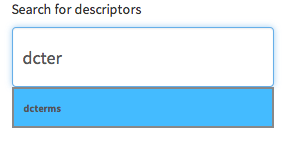
\includegraphics[width=0.4\textwidth]{Images/ontology_autocomplete}	
%	\caption{Typing to select a metadata schema}
%	\label{fig:ontology_autocomplete}
%\end{figure}
%
%After selecting the ``dcterms'' result from the list you will be presented with all the descriptors present in that schema. When you click on a descriptor it will be added to the main metadata editor at the center. Fill in each descriptor and press the ``Save'' button. You can undo the changes to the metadata record at any time by pressing the ``Undo'' button; to clear all the currently saved metadata, select the ``Clear'' button (Figure \ref{fig:metadata_editor_buttons}).
%
%\begin{figure}[h!t!]
%	\centering
%	
\includegraphics[width=0.8\textwidth]{Images/metadata_editor_buttons}	
%	\caption{Buttons available in the metadata editor}
%	\label{fig:metadata_editor_buttons}
%\end{figure}
%
%% subsubsection adding_descriptors_manually (end)
%
%% FORA
%\subsubsection{Semi-automated descriptor selection} % (fold)
%\label{ssub:semi_automated_descriptor_selection}
%
%As you interact with Dendro, the system will try to learn your descriptor preferences. The ``Usage-based'' descriptor selection mode (Figure \ref{fig:dendro_in_edit_mode}, area \textbf{4}) is activated by clicking the corresponding button, allowing you to select descriptors from a list of recommendations. If you do not find any of the suggested descriptors relevant, you may select the ``Previous page'' and ``Next page'' options to cycle through additional recommendations. This interaction itself will be taken into account, so next time the list of descriptors at the top may be more interesting. Figure \ref{fig:semi_automated_descriptor_selection} also shows the manual descriptor search box, which allows you to find additional descriptors by typing a part of their title or description. When you select a result from the hit list, the corresponding descriptor will be added to the metadata editor so that you can fill in the corresponding value.
%
%By selecting the ``Favorite'' button, (\raisebox{-4pt}{
\includegraphics[height=14pt]{images/favorite_descriptor}}), that particular descriptor will be bookmarked to be always visible. By selecting the ``Hide'' button (\raisebox{-4pt}{
\includegraphics[height=14pt]{images/hide_descriptor}}), the descriptor will not be shown at the top of the results page. You can find them again by browsing through the descriptor recommendation pages again.
%
%\begin{figure}[h!t!]
%	\centering
%	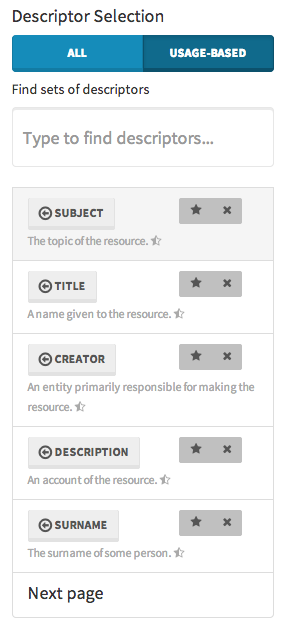
\includegraphics[width=0.4\textwidth]{Images/semi_automated_descriptor_selection}	
%	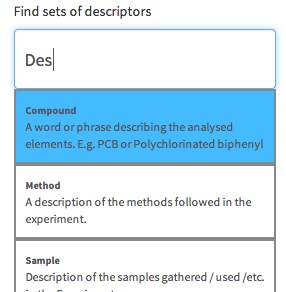
\includegraphics[width=0.4\textwidth]{Images/descriptor_autocomplete}	
%	\caption{Changing to the ``Usage-based'' mode for descriptor selection and searching for descriptors}
%	\label{fig:semi_automated_descriptor_selection}
%\end{figure}
%
%% subsubsection semi_automated_descriptor_selection (end)
%
%
%% subsection editing_metadata (end)
%
%\subsection{Viewing metadata editing history} % (fold)
%\label{sub:viewing_metadata_editing_history}
%
%\begin{figure}[h!t!]
%	\centering
%	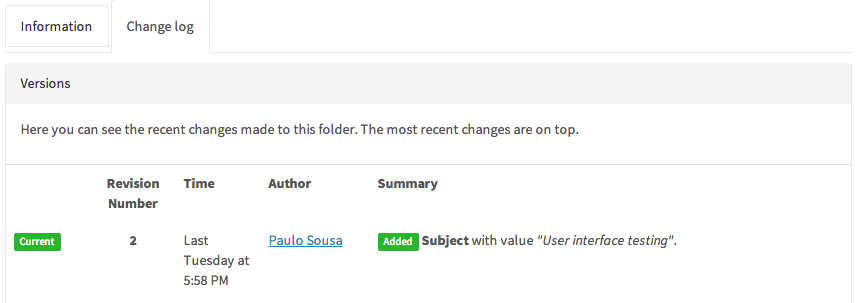
\includegraphics[width=\textwidth]{Images/change_log}	
%	\caption{Viewing the change log for a resource}
%	\label{fig:change_log}
%\end{figure}
%
%
%By selecting the ``Change log'' option in the metadata editor at the center you will be able to see the complete list of changes done to a currently selected resource. The list of changes will include the time of each modification, its author, which descriptors were changed and their new values (Figure \ref{fig:change_log}).
%
%% subsection viewing_metadata_editing_history (end)
%
%\subsection{Backup and restore your data and metadata} % (fold)
%\label{sub:backup_and_restore_your_data_and_metadata}
%
%You may want do download an entire folder for your own personal backups, you can do so by pressing the ``Backup'' button (\raisebox{-4pt}{
\includegraphics[height=14pt]{images/buttons/backup}}). The currently open folder will be compressed into a ZIP file that will start to be downloaded. Not only the data (file structure) will be backed up, but also the entire struture's metadata records. 
%
%The ``Restore'' operation will allow you to select a ZIP file and upload it to the Dendro system. The contents will be extracted and loaded into the system, replacing the contents of the currently open folder. You can use this not only to roll back a folder to a previous state, but also to upload several files at once, as follows: organize your directory structure in your own desktop computer and then compress them into a ZIP file; then simply send it through the restore function; wait for the restore operation to complete (it may take a while) and then you will see a copy of the entire structure represented in Dendro. You can then edit the metadata values for each folder and file using the metadata editor. 
%
%If the ZIP file sent in for the restoring operation was produced by a Dendro backup procedure and not manually by you, it will contain the metadata associated to the original folder structure at the time. That metadata will also be restored along with the file structure.
%
%% subsection backup_and_restore_your_data_and_metadata (end)

%FORA

%\subsection{Sharing your dataset} % (fold)
%\label{sub:sharing_your_dataset}
%
%Dendro is designed to be a collaborative ``staging area'' for bringing data and metadata together so that they can be shared, hence complementing research publications. 
%
%The ``Share'' button allows you to connect to a repository of your choosing (DSpace\footnote{\url{http://www.dspace.org}}, CKAN\footnote{\url{http://ckan.org}}, EPrints\footnote{\url{http://www.eprints.org}}, Figshare\footnote{\url{http://figshare.com}} and Zenodo\footnote{\url{http://zenodo.org}} are supported). After creating a repository bookmark for the platform, it will be saved for future reuse, so that you do not need to fill in the details every time you wish to share a dataset. This platform may be the institutional repository of your University, for example. Figure \ref{fig:share_screens} shows how you may need to input different information that is necessary for the sharing of  share datasets to different types of respositories. When in doubt, please contact your insitution's repository administrator to know how you can send data from Dendro to it.
%
%Regardless of the repository you choose, the data that will be shared will be the files that are contained in the \textbf{currently open folder}. The metadata that will be associated to the new item will be the one that is associated to that folder too.
%
%\begin{figure}[h!t!]
%	\centering
%	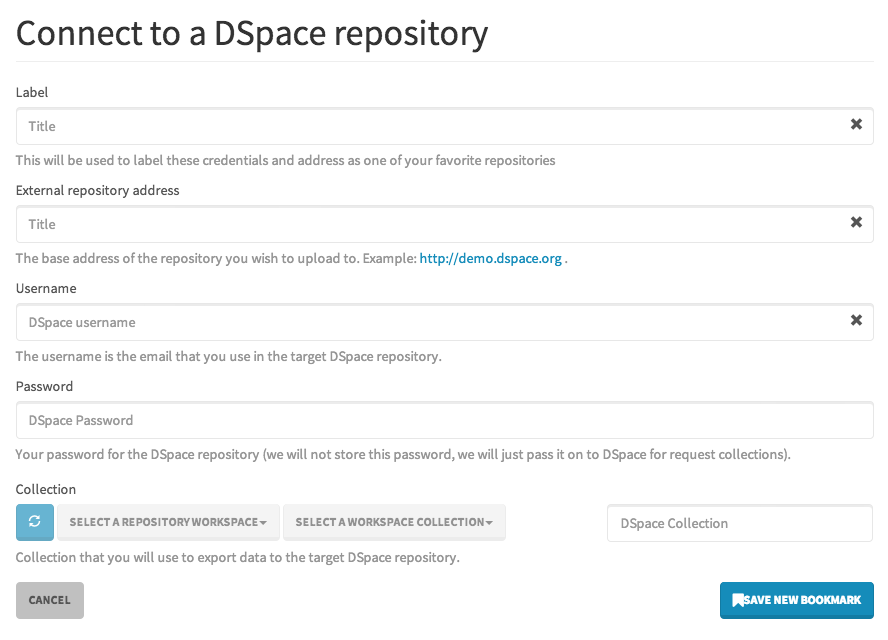
\includegraphics[width=0.3\textwidth]{Images/shares/dspace}	
%	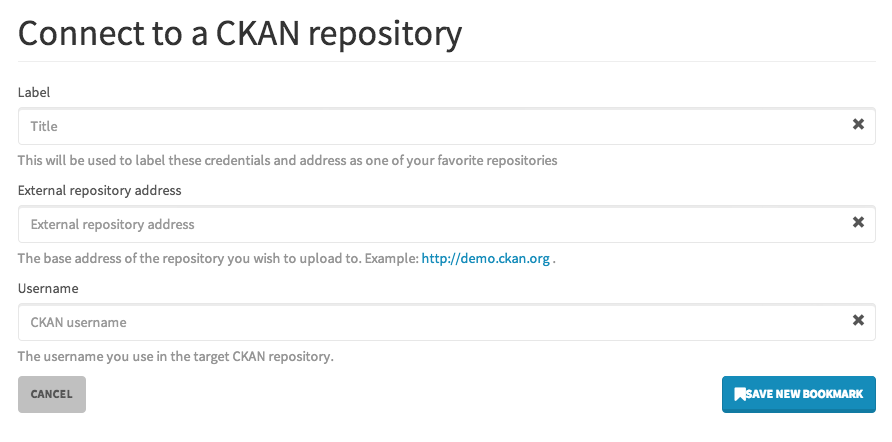
\includegraphics[width=0.3\textwidth]{Images/shares/ckan}	
%	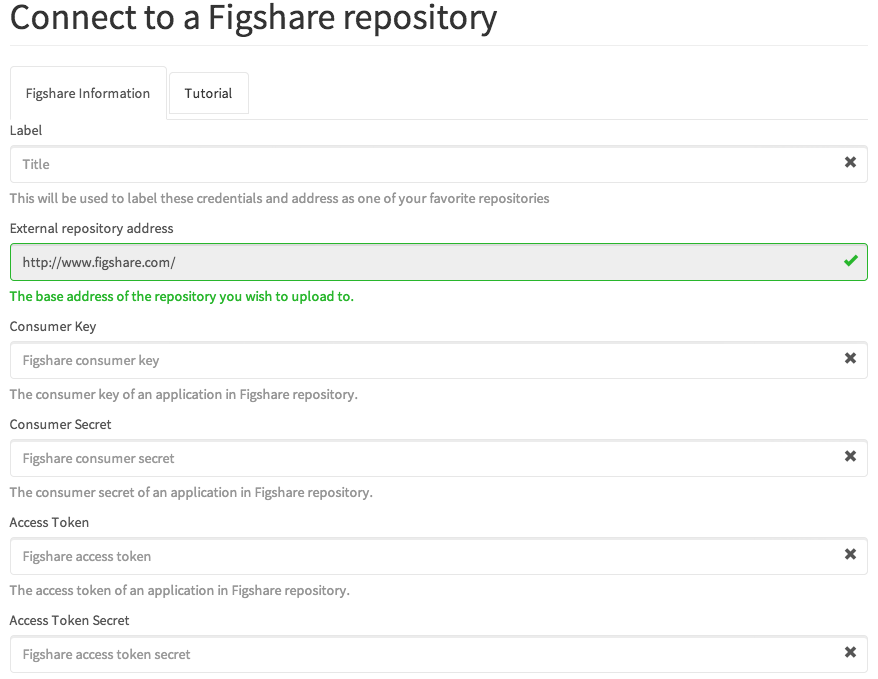
\includegraphics[width=0.3\textwidth]{Images/shares/figshare}	
%	\caption{Sharing to different repositories requires different information}
%	\label{fig:share_screens}
%\end{figure}
%
%% subsection sharing_your_dataset (end)
%
%% section managing_files_and_creating_metadata_records (end)
%
%\section{A call for opinions} % (fold)
%\label{sec:a_call_for_opinions}
%
%The interactions that are currently being recorded as a way to improve the descriptor recommendation mechanisms are the following:
%
%\begin{enumerate}
%	\item Selection of a descriptor from the recommendations list
%	\item Saving a descriptor with a non-empty value
%	\item Favoriting a descriptor
%	\item Hiding a descriptor
%	\item Filling in a descriptor in the metadata editor, as long as it was recommended (Recommendations ON button is active)
%	\item Browsing to the Next/Previous pages in the list of descriptor recommendations
%	\item Manually selecting a given ontology
%	\item Selecting a descriptor from the manual selection list
%\end{enumerate}
%
%If you have any ideas about possible interactions that could be used as source of evidence for determining if a researcher favours a certain descriptor or set of descriptors, please feel free to contact us. We would be glad to include that evidence in the ranking formula and see if the descriptor recommendations become even better!
%
%% section a_call_for_opinions (end)

\vspace*{\fill}
\begin{center}
\begin{minipage}{.6\textwidth}
Este guião mostra as funcionalidades mais usadas no Dendro por um curador de dados. A partir daqui pode explorar a plataforma e, em caso de \emph{erros}, problemas ou dúvidas use o fórum Moodle da Unidade Curricular ou o email:\\\url{mailto:joaorosilva@gmail.com}. 

\textbf{Bom trabalho!}


\end{minipage}
\end{center}
\vfill % equivalent to \vspace{\fill}

\end{document}